% Hình: Khối RDMS - Residual Dilated Multi-Scale (Mục 4.3)
\documentclass[border=6pt]{standalone}
\usepackage[utf8]{vietnam}
\usepackage{amsmath,amssymb}
\usepackage{xcolor}
\usepackage{tikz}
\usetikzlibrary{positioning,fit,arrows.meta,calc,backgrounds}
\definecolor{cvblue}{HTML}{35618E}\definecolor{cvbluefill}{HTML}{DCE7F2}
\definecolor{slate}{HTML}{5B6470}\definecolor{slatefill}{HTML}{EDEFF2}
\definecolor{lssorange}{HTML}{CF8A2A}\definecolor{lssfill}{HTML}{FBE7C6}
\definecolor{inkdark}{HTML}{23272E}
\tikzset{
  >={Stealth[length=2.4mm]},
  every node/.style={font=\sffamily\footnotesize, text=inkdark},
  blk/.style={draw=cvblue, fill=cvbluefill, rounded corners=2pt, thick, align=center, minimum height=8mm, minimum width=22mm},
  br/.style={draw=cvblue, fill=white, rounded corners=2pt, thick, align=center, minimum height=8mm, minimum width=26mm},
  io/.style={draw=slate, rounded corners=2pt, thick, align=center, minimum height=8mm, minimum width=13mm},
  op/.style={draw=lssorange, fill=lssfill, circle, thick, inner sep=1pt, minimum size=6.5mm},
  flow/.style={-{Stealth[length=2.4mm]}, line width=0.9pt, draw=inkdark},
  lbl/.style={font=\sffamily\scriptsize, text=slate},
}
\begin{document}
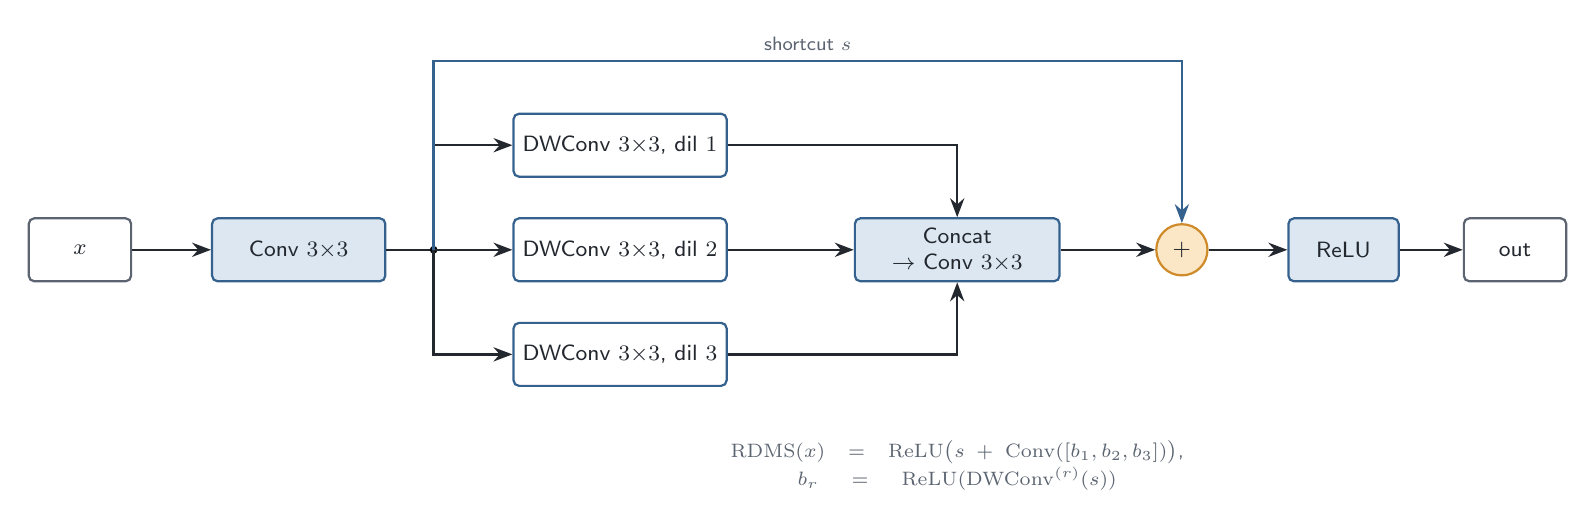
\begin{tikzpicture}
  \node[io] (x) {$x$};
  \node[blk, right=10mm of x] (sc) {Conv $3{\times}3$};
  \node[br, right=16mm of sc] (b2) {DWConv $3{\times}3$, dil $2$};
  \node[br, above=5mm of b2] (b1) {DWConv $3{\times}3$, dil $1$};
  \node[br, below=5mm of b2] (b3) {DWConv $3{\times}3$, dil $3$};
  \node[blk, right=16mm of b2, minimum width=26mm] (cat) {Concat\\ $\to$ Conv $3{\times}3$};
  \node[op, right=12mm of cat] (add) {$+$};
  \node[blk, right=10mm of add, minimum width=14mm] (relu) {ReLU};
  \node[io, right=8mm of relu] (out) {out};

  \draw[flow] (x) -- (sc);
  \coordinate (s) at ($(sc.east)+(6mm,0)$);
  \draw[flow,-] (sc) -- (s); \fill (s) circle (1.4pt);
  \draw[flow] (s) |- (b1.west);
  \draw[flow] (s) -- (b2.west);
  \draw[flow] (s) |- (b3.west);
  \draw[flow] (b1.east) -| (cat.north);
  \draw[flow] (b2.east) -- (cat.west);
  \draw[flow] (b3.east) -| (cat.south);
  \draw[flow] (cat) -- (add);
  \draw[flow] (add) -- (relu);
  \draw[flow] (relu) -- (out);
  
  % shortcut phần dư (Đã nâng độ cao lên 24mm để không bị cắt qua ô b1)
  \draw[flow, draw=cvblue] (s) -- ++(0,24mm) coordinate (s_top) 
        -- (s_top -| add.north) node[midway, above, lbl]{shortcut $s$} 
        -- (add.north);
        
  % Đã chỉnh lại vị trí neo theo đáy b3 để tránh đè lên đường nối
  \node[lbl] at ($(cat |- b3.south) - (0, 10mm)$) [text width=8.5cm, align=center]
        {$\mathrm{RDMS}(x)=\mathrm{ReLU}\big(s+\mathrm{Conv}([b_1,b_2,b_3])\big)$, \ $b_r=\mathrm{ReLU}(\mathrm{DWConv}^{(r)}(s))$};
\end{tikzpicture}
\end{document}